\documentclass{article}

%!TEX root = article.tex
\usepackage[utf8]{inputenc}
\usepackage[T1]{fontenc}

% Bold math
\usepackage{bm}
\usepackage{dsfont}
\usepackage{csquotes}

% Micro-typing
\usepackage{xspace}
\usepackage{nicefrac}
\usepackage[super]{nth}
\usepackage{microtype}

\usepackage{multibib}

\usepackage[english]{babel}

% Compact itemize
\usepackage{enumitem}

% Tables
\usepackage{booktabs}
\usepackage{makecell}


\usepackage{graphicx}
\graphicspath{{./figures/}}

\usepackage{subcaption}

% For colors
\usepackage{xcolor}

% Algorithm
\usepackage{algorithm}
\usepackage[noend]{algpseudocode}
\algrenewcommand{\algorithmiccomment}[1]{$\vartriangleright$ #1}
\algrenewcommand{\algorithmicreturn}{\textbf{Return: }}
\algnewcommand\algorithmicinput{\textbf{Input: }}
\algnewcommand\Input{\State \algorithmicinput}

% Hyper reference
\usepackage[colorlinks=true,bookmarks=true,linkcolor=blue,
urlcolor=blue,citecolor=blue,breaklinks=true]{hyperref}

\usepackage{url}

\makeatletter
\addto\extrasenglish{%
\renewcommand{\appendixautorefname}{App.}%
\renewcommand{\figureautorefname}{Fig.}%
\renewcommand{\tableautorefname}{Table}%
\renewcommand{\sectionautorefname}{\S\@gobble}%
\renewcommand{\subsectionautorefname}{\S\@gobble}%
\renewcommand{\subsubsectionautorefname}{\S\@gobble}%
}
\makeatother

% Float parameters, for more full pages.
\renewcommand{\topfraction}{0.9}	% max fraction of floats at top
\renewcommand{\bottomfraction}{0.8}	% max fraction of floats at bottom
\renewcommand{\textfraction}{0.07}	% allow minimal text w. figs
%   Parameters for FLOAT pages (not text pages):
\renewcommand{\floatpagefraction}{0.6}	% require fuller float pages
%    % N.B.: floatpagefraction MUST be less than topfraction !!
\renewcommand{\dbltopfraction}{.95}  % double page floats at the top
\renewcommand{\dblfloatpagefraction}{.6}
\setcounter{totalnumber}{4}
\setcounter{topnumber}{3}
\setcounter{dbltopnumber}{3}
\setcounter{bottomnumber}{2}

% Wide pages for supplementary figures
\usepackage{changepage}                 % adjust margins for selected portions
% wide page for side by side figures, tables, etc
\newlength{\offsetpage}
\setlength{\offsetpage}{3.0cm}
\newenvironment{widepage}{\begin{adjustwidth}{-\offsetpage}{-\offsetpage}%
    \addtolength{\textwidth}{2\offsetpage}}%
{\end{adjustwidth}}


% MATHS (AMS)
\usepackage{amsmath}
\usepackage{amsfonts} 
\usepackage{amssymb}
\usepackage{mathrsfs}
\usepackage{mathtools} % for psmallmatrix
\mathtoolsset{showonlyrefs}

\usepackage{amsthm}

\newtheorem{theorem}{Theorem}
\newtheorem{proposition}{Proposition}
\newtheorem{definition}{Definition}
\newtheorem{corollary}{Corollary}
\newtheorem{lemma}{Lemma}
\newtheorem{remark}{Remark}
\newtheorem{example}{Example}
\newtheorem{assumption}{Assumption}

\newtheorem{subassumptioninner}{Assumption}
\newenvironment{subassumption}[1]{%
  \renewcommand\thesubassumptioninner{#1}%
  \subassumptioninner
}{\endsubassumptioninner}

\newcommand{\definitionautorefname}{Def.}%
\newcommand{\propositionautorefname}{Prop.}%
\newcommand{\corollaryautorefname}{Corollary}%
\newcommand{\assumptionautorefname}{Ass.}%
\newcommand{\subassumptioninnerautorefname}{Ass.}%
\newcommand{\algorithmautorefname}{Alg.}%
\newcommand{\lemmaautorefname}{Lemma}
\newcommand{\remarkautorefname}{Rmk.}

\newcommand{\todo}[1]{{\color{red} TODO: #1}}

%!TEX root = notes.tex
%% Symboles avec double lignes
\newcommand{\NN}{\mathbb{N}}
\newcommand{\CC}{\mathbb{C}}
\newcommand{\GG}{\mathbb{G}}
\newcommand{\LL}{\mathbb{L}}
\newcommand{\PP}{\mathbb{P}}
\renewcommand{\SS}{\mathbb{S}}
\newcommand{\QQ}{\mathbb{Q}}
\newcommand{\RR}{\mathbb{R}}
\newcommand{\VV}{\mathbb{V}}
\newcommand{\ZZ}{\mathbb{Z}}
\newcommand{\FF}{\mathbb{F}}
\newcommand{\KK}{\mathbb{K}}
\newcommand{\TT}{\mathbb{T}}
\newcommand{\UU}{\mathbb{U}}
\newcommand{\EE}{\mathbb{E}}
\newcommand{\XX}{\mathbb{X}}
\newcommand{\YY}{\mathbb{Y}}
%% Symboles arrondis
\newcommand{\Aa}{\mathcal{A}}
\newcommand{\Bb}{\mathcal{B}}
\newcommand{\Cc}{\mathcal{C}}
\newcommand{\Dd}{\mathcal{D}}
\newcommand{\Ee}{\mathcal{E}}
\newcommand{\Ff}{\mathcal{F}}
\newcommand{\Gg}{\mathcal{G}}
\newcommand{\Hh}{\mathcal{H}}
\newcommand{\Ii}{\mathcal{I}}
\newcommand{\Jj}{\mathcal{J}}
\newcommand{\Kk}{\mathcal{K}}
\newcommand{\Ll}{\mathcal{L}}
\newcommand{\Mm}{\mathcal{M}}
\newcommand{\Nn}{\mathcal{N}}
\newcommand{\Oo}{\mathcal{O}}
\newcommand{\Pp}{\mathcal{P}}
\newcommand{\Qq}{\mathcal{Q}}
\newcommand{\Rr}{\mathcal{R}}
\newcommand{\Ss}{\mathcal{S}}
\newcommand{\Tt}{\mathcal{T}}
\newcommand{\Uu}{\mathcal{U}}
\newcommand{\Vv}{\mathcal{V}}
\newcommand{\Ww}{\mathcal{W}}
\newcommand{\Xx}{\mathcal{X}}
\newcommand{\Yy}{\mathcal{Y}}
\newcommand{\Zz}{\mathcal{Z}}
\newcommand{\KL}{\text{KL}}

% matrices
\newcommand{\A}{\bm{A}}
\newcommand{\B}{\bm{B}}
\newcommand{\C}{\bm{C}}
\newcommand{\D}{\bm{D}}
\newcommand{\E}{\bm{E}}
\newcommand{\F}{\bm{F}}
\newcommand{\G}{\bm{G}}
\newcommand{\Hz}{\bm{H}}
\newcommand{\I}{\bm{I}}
\newcommand{\J}{\bm{J}}
\newcommand{\K}{\bm{K}}
\newcommand{\Lz}{\bm{L}}
\newcommand{\M}{\bm{M}}
\newcommand{\N}{\bm{N}}
\newcommand{\Oz}{\bm{O}}
\newcommand{\Pz}{\bm{P}}
\newcommand{\Q}{\bm{Q}}
\newcommand{\R}{\bm{R}}
\newcommand{\Sz}{\bm{S}}
\newcommand{\T}{\bm{T}}
\newcommand{\U}{\bm{U}}
\newcommand{\V}{\bm{V}}
\newcommand{\W}{\bm{W}}
\newcommand{\X}{\bm{X}}
\newcommand{\Y}{\bm{Y}}
\newcommand{\Z}{\bm{Z}}

% Vectors
\renewcommand{\a}{\bm{a}}
\renewcommand{\b}{\bm{b}}
\renewcommand{\c}{\bm{c}}
\renewcommand{\d}{\textrm{d}}
\newcommand{\e}{\bm{e}}
\newcommand{\f}{\bm{f}}
\newcommand{\g}{\bm{g}}
\newcommand{\h}{\bm{h}}
\renewcommand{\i}{\bm{i}}
\renewcommand{\j}{\bm{j}}
\renewcommand{\k}{\bm{k}}
\renewcommand{\l}{\bm{l}}
\newcommand{\m}{\bm{m}}
\newcommand{\n}{\bm{n}}
\renewcommand{\o}{\bm{o}}
\newcommand{\p}{\bm{p}}
\newcommand{\q}{\bm{q}}
\renewcommand{\r}{\bm{r}}
\newcommand{\s}{\bm{s}}
\renewcommand{\t}{\bm{t}}
\renewcommand{\u}{\bm{u}}
\renewcommand{\v}{\bm{v}}
\newcommand{\w}{\bm{w}}
\newcommand{\x}{\bm{x}}
\newcommand{\y}{\bm{y}}
\newcommand{\z}{\bm{z}}

% greek
\newcommand{\al}{\alpha}
\newcommand{\la}{\lambda}
\newcommand{\ga}{\gamma}
\newcommand{\Ga}{\Gamma}
\newcommand{\La}{\Lambda}
\newcommand{\si}{\sigma}
%\newcommand{\Si}{\Sigma}
\newcommand{\be}{\beta}
\newcommand{\de}{\delta}
\newcommand{\De}{\Delta}
\renewcommand{\phi}{\varphi}
\renewcommand{\th}{\theta}
\newcommand{\om}{\omega}
\newcommand{\Om}{\Omega}

% hat, tilde
\newcommand{\hf}{\hat f}
\newcommand{\wtf}{\tilde f}
\newcommand{\tx}{\tilde x}
\newcommand{\ta}{\tilde a}
\newcommand{\tb}{\tilde b}
\newcommand{\ty}{\tilde y}
\newcommand{\tu}{\tilde u}
\newcommand{\tv}{\tilde v}
\newcommand{\tga}{\tilde \ga}
\newcommand{\tf}{\wt{f}}



%%%%%%%%%%%%%%% MATHS OPERATORS %%%%%%%%%%%%%%%%%
\newcommand{\ins}[1]{\mathrm{#1}}

\DeclareMathOperator{\realp}{\Rr e}
\DeclareMathOperator{\imagp}{\Ii m}
\DeclareMathOperator{\Ker}{Ker}
\DeclareMathOperator{\Hom}{Hom}
\DeclareMathOperator{\End}{End}
\DeclareMathOperator{\tr}{tr}
\DeclareMathOperator{\Tr}{Tr}
\DeclareMathOperator{\Supp}{Supp}
\DeclareMathOperator{\Sign}{Sign}
\let\Im\relax
\DeclareMathOperator{\Im}{Im}
\DeclareMathOperator{\Corr}{Corr}
\DeclareMathOperator{\sign}{sign}
\DeclareMathOperator{\supp}{supp}

\DeclareMathOperator{\cas}{cas}
\DeclareMathOperator{\sinc}{sinc}
\DeclareMathOperator{\cotan}{cotan}
\DeclareMathOperator{\Card}{Card}
\DeclareMathOperator{\GCD}{GCD}
\DeclareMathOperator{\grad}{grad}
\DeclareMathOperator{\Diag}{Diag}
\DeclareMathOperator{\rank}{rank}
\DeclareMathOperator{\conv}{conv}
\DeclareMathOperator{\interop}{int}

\newcommand{\ps}[2]{\langle #1,#2\rangle}

% regularity
\newcommand{\Calpha}{\mathrm{C}^\al}
\newcommand{\Cbeta}{\mathrm{C}^\be}
\newcommand{\Cal}{\text{C}^\al}
\newcommand{\Ctwo}{\text{C}^{2}}
\newcommand{\Calt}[1]{\text{C}^{#1}}
\newcommand{\Cder}[1]{\mathscr{C}^{#1}}
% Lp spaces
\newcommand{\lone}{\ell^1}
\newcommand{\ltwo}{\ell^2}
\newcommand{\linf}{\ell^\infty}
\newcommand{\Lone}{\text{\upshape L}^1}
\newcommand{\Ltwo}{\text{\upshape L}^2}
\newcommand{\Linf}{\text{\upshape L}^\infty}
\newcommand{\lzero}{\ell^0}
\newcommand{\lp}{\ell^p}
% circle
\newcommand{\Sun}{\text{S}^1}
% little space after forall
\newcommand{\foralls}{\forall \,}
%% for derivatives
\newcommand{\dd}{\ins{d}}
%% Use french comparaison operator
\renewcommand{\leq}{\leqslant}
\renewcommand{\geq}{\geqslant}


%%%%%%%%%%%%%%% MATHS CONSTRUCTS %%%%%%%%%%%%%%%

%% over-symbols
\newcommand{\ol}[1]{\overline{#1}}
\newcommand{\wh}[1]{\widehat{#1}}
\newcommand{\whwh}[1]{\hat{\hat{#1}}}
\newcommand{\wt}[1]{\widetilde{#1}}
%% partial derivatives
\newcommand{\pd}[2]{ \frac{ \partial #1}{\partial #2} }
\newcommand{\pdd}[2]{ \frac{ \partial^2 #1}{\partial #2^2} }
%% nice epsilon
\renewcommand{\epsilon}{\varepsilon}
%% Pour avoir un joli i pour les complexes
\renewcommand{\imath}{\mathrm{i}}
\newcommand{\interior}[1]{\ensuremath{\overset{\circ}{#1}}}

%% Legendre symbol
\newcommand{\legsymb}[2]{ \genfrac{(}{)}{}{}{#1}{#2} }
%% exposant pour les ordinaux
\newcommand{\ordin}[2]{ ${#1}^{ \text{#2} }$ }
%% Dot product and cross product
% \newcommand{\dotp}[2]{ \left\langle #1,\,#2 \right\rangle }
\newcommand{\dotp}[2]{\langle #1,\,#2\rangle}
\newcommand{\dotps}[2]{\langle #1,\,#2\rangle}
\newcommand{\crossp}[2]{ #1 \hat #2 }
\newcommand{\seg}[2]{\llbracket #1,\,#2 \rrbracket}
\newcommand{\brac}[1]{\left[#1\right]}
%\newcommand{\norm}[1]{|\!| #1 |\!|}
\newcommand{\norm}[1]{\left\| #1 \right\|}
\newcommand{\snorm}[1]{\| #1 \|}
\newcommand{\normb}[1]{\Big|\!\Big| #1 \Big |\!\Big|}
\newcommand{\normB}[1]{\left|\!\left| #1 \right|\!\right|}
\DeclareMathOperator{\diverg}{div}
\DeclareMathOperator{\Prox}{Prox}
\newcommand{\normT}[1]{\norm{#1}_{\text{T}}}
\newcommand{\normu}[1]{\norm{#1}_{1}}
\newcommand{\normi}[1]{\norm{#1}_{\infty}}
\newcommand{\normd}[1]{\norm{#1}_{2}}
\newcommand{\normz}[1]{\norm{#1}_{0}}
\newcommand{\abs}[1]{\left\lvert#1\right\rvert} % modified by Vincent
\newcommand{\absb}[1]{\Big| #1 \Big|}

%% Function definition
\newcommand{\func}[4]{ {\left\{  \begin{array}{ccc} #1 & \longrightarrow & #2 \\ #3 & \longmapsto & #4 \end{array}  \right.} }
% transpose
\newcommand{\transp}[1]{ {#1}^{\ins{T}} }
% l'identit�
\newcommand{\Id}{\ins{Id}}
% egal par d�finition
\newcommand{\eqdef}{\triangleq}

\DeclareMathOperator*{\argmin}{argmin}
\DeclareMathOperator*{\argmax}{argmax}
% \DeclareMathOperator*{\sup}{sup}

%% parenthesis
\newcommand{\pa}[1]{\left( #1 \right)}
\newcommand{\bpa}[1]{\big( #1 \big)}
\newcommand{\choice}[1]{ %
	\left\{ %
		\begin{array}{l} #1 \end{array} %
	\right. }
% ensembles
\newcommand{\set}[1]{ \{ #1 \} }
\newcommand{\condset}[2]{ \left\{ #1 \;;\; #2 \right\} }


%%%%%%%%%%%%%%% SPACES %%%%%%%%%%%%%%%%%
\newcommand{\qandq}{ \quad \text{and} \quad }
\newcommand{\qqandqq}{ \qquad \text{and} \qquad }
\newcommand{\qifq}{ \quad \text{if} \quad }
\newcommand{\qqifqq}{ \qquad \text{if} \qquad }
\newcommand{\qwhereq}{ \quad \text{where} \quad }
\newcommand{\qqwhereqq}{ \qquad \text{where} \qquad }
\newcommand{\qwithq}{ \quad \text{with} \quad }
\newcommand{\qqwithqq}{ \qquad \text{with} \qquad }
\newcommand{\qforq}{ \quad \text{for} \quad }
\newcommand{\qqforqq}{ \qquad \text{for} \qquad }
\newcommand{\qqsinceqq}{ \qquad \text{since} \qquad }
\newcommand{\qsinceq}{ \quad \text{since} \quad }
\newcommand{\qarrq}{\quad\Longrightarrow\quad}
\newcommand{\qqarrqq}{\quad\Longrightarrow\quad}
\newcommand{\qiffq}{\quad\Longleftrightarrow\quad}
\newcommand{\qqiffqq}{\qquad\Longleftrightarrow\qquad}
\newcommand{\qsubjq}{ \quad \text{subject to} \quad }
\newcommand{\qqsubjqq}{ \qquad \text{subject to} \qquad }
\newcommand{\qobjq}[1]{\quad \text{#1} \quad}
\newcommand{\qqobjqq}[1]{\quad \text{#1} \quad}



% Restrictions
% Exemple: $ \rest{f}{ \Z } $

\newlength{\restsubwidth}
\newlength{\restsubheight}
\newlength{\restsubmoreheight}
\setlength{\restsubmoreheight}{4pt}
\newcommand{\rest}[2]{%
        \settowidth{\restsubwidth}{\ensuremath{#2}}
        \settoheight{\restsubheight}{\ensuremath{{}_{#2}}}
        \ensuremath{{#1\hskip 0.5pt}_{\vrule\kern2pt\parbox[b][%
        4pt][b]{\the\restsubwidth}{%
                        \ensuremath{{}_{#2}}}}}
        }

% \renewcommand*{\bibfont}{\small}
\graphicspath{{./figures/}}

\usepackage{icml2020}

% If accepted, instead use the following line for the camera-ready submission:
%\usepackage[accepted]{icml2020}

% The \icmltitle you define below is probably too long as a header.
% Therefore, a short form for the running title is supplied here:
\icmltitlerunning{Online Sinkhorn: optimal transportation distances from sample streams}

\begin{document}

\twocolumn[
\icmltitle{Online Sinkhorn: optimal transportation distances from sample streams}

% It is OKAY to include author information, even for blind
% submissions: the style file will automatically remove it for you
% unless you've provided the [accepted] option to the icml2020
% package.

% List of affiliations: The first argument should be a (short)
% identifier you will use later to specify author affiliations
% Academic affiliations should list Department, University, City, Region, Country
% Industry affiliations should list Company, City, Region, Country

% You can specify symbols, otherwise they are numbered in order.
% Ideally, you should not use this facility. Affiliations will be numbered
% in order of appearance and this is the preferred way.
\icmlsetsymbol{equal}{*}

\begin{icmlauthorlist}
\icmlauthor{Arthur Mensch}{ens}
\icmlauthor{Gabriel Peyré}{ens}
\end{icmlauthorlist}

\icmlaffiliation{ens}{ENS, DMA, Paris, France}

\icmlcorrespondingauthor{Arthur Mensch}{arthur.mensch@m4x.org}

% You may provide any keywords that you
% find helpful for describing your paper; these are used to populate
% the "keywords" metadata in the PDF but will not be shown in the document
\icmlkeywords{Non-convex optimisation, game theory, GANs}

\vskip 0.3in
]

\printAffiliationsAndNotice{}  % leave blank if no need to mention equal contribution
% \printAffiliationsAndNotice{\icmlEqualContribution} % otherwise use the standard text.

\begin{abstract}
  Optimal Transport (OT) distances are now routinely used as loss functions in ML tasks. Yet, computing OT distances between arbitrary (i.e. not necessarily discrete) probability distributions remains an open problem. This paper introduces a new online estimator of entropy-regularized OT distances between two such arbitrary distributions. It uses streams of samples from both distributions to iteratively enrich a non-parametric representation of the transportation plan. Compared to the classic Sinkhorn algorithm, our method leverages new samples at each iteration, which enables a consistent estimation of the true regularized OT distance. We cast our algorithm as a block-convex mirror descent in the space of positive distributions, and provide a theoretical analysis of its convergence. We numerically illustrate the performance of our method in comparison with concurrent approaches.
\end{abstract}

%!TEX root = article.tex

Optimal transport (OT) distances are fundamental in statistical learning, both
as a tool for analyzing the convergence of various
algorithms~\citep{canas2012learning,dalalyan2019user}, and as a data-dependent
term for tasks as diverse as supervised learning~\citep{frogner2015learning},
unsupervised generative modeling~\citep{arjovsky2017wgan} or domain
adaptation~\citep{courty2016optimal}.
%
OT lifts a given distance over data points living in space $\Xx$ into a distance
on the space $\Pp(\Xx)$ of probability distributions over this data space $\Xx$. We refer to the monograph of~\citet{santambrogio2015optimal} for a detailed mathematical treatment.
%
This distance has many favorable geometrical properties. In particular it allows one to compare distributions having disjoint supports. 
% 
Computing OT distance is usually performed by sampling once from the input
distributions and solving a discrete linear program (LP), due
to~\citet{Kantorovich42}. This approach is numerically costly and statistically
inefficient \citep{weed2019sharp}. The optimisation problem depends on a fixed
sampling of points from the data. It is therefore not adapted to machine
learning setting where data is resampled continuously (e.g. in GANs), or
accessed in an online manner. The goal of this paper is to develop an efficient
online method able to estimate OT distances between continuous distributions. We
will use a stream of data to refine an approximate optimal transport solution,
adapting the celebrated Sinkhorn algorithm to an online setting.
  


%%%%
To alleviate both the computational and statistical burdens of OT, it is common
to regularize the Kantorovich LP.
%
The most successful approach in this direction is to use an entropic barrier penalty. 
%
When dealing with discrete distributions, this yields a problem that can be solved
numerically using Sinkhorn-Knopp's matrix balancing
algorithm~\citep{Sinkhorn64,sinkhorn1967concerning}.
%
This approach was pushed forward for ML applications by
\citet{cuturi2013sinkhorn}. Sinkhorn distances are smooth and amenable to GPU
computations, which makes them suitable as a loss function in model training.
The Sinkhorn algorithm operates in two distinct phases: draw samples from the
distributions and evaluate a pairwise distance matrix in the first phase;
balance this distance matrix using Sinkhorn-Knopp iterations in the second
phase.

This two-step approach does not estimate the true regularized OT
distance, and cannot handle samples provided as a stream, e.g. renewed at each
training iteration of an outer algorithm. A cheap fix is to use Sinkhorn over
mini-batches (see for instance~\citet{2018-Genevay-aistats} for an application
to GANs). Yet this introduces a strong estimation bias, especially in high
dimension ---see~\citet{fatras2019learning} for a mathematical analysis. In
contrast, we use streams of mini-batches to progressively enrich a consistent representation of the
transport plan.

\paragraph{Contributions.} Our paper proposes a new take on estimating optimal transport distances between continuous distributions. We make the following contribution
\begin{itemize}
    \item We introduce an online variant of the Sinkhorn algorithm, that uses
    streams of samples $(x_t)_t$ and $(y_t)_y$ to enrich a non-parametric
    functional representation of the dual regularized optimal transport solution.
    \item We cast online Sinkhorn as an instance of a block-convex stochastic mirror
    descent algorithm. This shows convergence of the algorithm
    with high probability. We analyse special cases of online Sinkhorn.
    \item We demonstrate the performance of online Sinkhorn for estimating OT
    distances between continuous distributions and for accelerating the early phase of discrete Sinkhorn iterations. Comparison with other methods advocates for our original non-parametric representations of OT solutions.
\end{itemize}

\paragraph{Notations.} We denote $\Cc(\Xx)$ the set of continuous functions over
a space $\Xx$, $\Mm^+(\Xx)$ and $\Pp(\Xx)$ the set of positive and probability
measures on $\Xx$, respectively. $\frac{d \mu}{d \alpha}$ denotes the
Radon-Nikodym derivative of measure $\mu$ with respect to measure $\alpha$. We
write $(i, j]$ the sequence $[i+1, \dots, j]$.


\section{Related work}\label{sec:related}

We review recent work on Sinkhorn distances and on the general problem of estimating optimal transport distances. 

\paragraph{Sinkhorn properties.} Sinkhorn algorithm computes $\epsilon$-accurate
approximations of OT in $O(n^2/\epsilon^3)$ operations for a number $n$ of
samples~\citep{altschuler2017near} (in contrast to the $O(n^3)$ complexity for an
exact solution). Moreover, these Sinkhorn distances does not suffers from the
curse of dimensionality~\citep{2019-Genevay-aistats}, since the average error
using $n$ random samples decays like $O(\epsilon^{-d/2}/\sqrt{n})$ in dimension
$d$, in sharp contrast with the slow $O(1/n^{1/d})$ error decay of
OT~\citep{dudley_speed_1969,weed2019sharp}. These Sinkhorn distances can furthermore be sharpened
by entropic debiasing~\citep{2019-Feydy-aistats}. Our work is rather orthogonal to these references, as it focuses on estimating distances between continuous distributions.

\paragraph{Continuous optimal transport.} Extending OT computations to arbitrary
distributions (possibly having continuous densities) without relying on a fixed
a priori sampling is an emerging topic of interest. A special case is the
semi-discrete setting, where one of the two distributions is discrete. Without
regularization, over an Euclidean space, this can be solved efficiently using
the computation of Voronoi-like diagrams~\citep{merigot2011multiscale}. This
idea can be extended to entropic-regularized OT~\citep{cuturi2018semidual}, and
can also be coupled with stochastic optimization
method~\citep{2016-genevay-nips} to tackle high dimensional problems (see
also~\citet{staib2017parallel} for an extension to Wasserstein barycenters). 

When dealing with arbitrary continuous densities, which are accessed through a
stream of random samples, the challenge is to approximate  the (continuous) dual
variables of the regularized Kantorovich LP using parametric or non-parametric
classes of functions. For application to generative model fitting, one can use
deep networks, which leads to an alternative formulation of Generative
Adversarial Networks (GANs)~\citep{arjovsky2017wgan} (see
also~\citet{seguy2018large} for an extension to the estimation of transportation
maps). There is however no theoretical guarantees for this type of dual
approximations, due to the non-convexity of the resulting optimization problem.
To our knowledge, the only mathematically rigorous algorithm uses reproducing
Hilbert space representations of potentials~\citep{2016-genevay-nips}. As this
construction is generic to all optimisation problems over functions, the convergence is slow. The representations we introduce outperform RKHS representations (\autoref{sec:compare}).

%!TEX root = article.tex

%!TEX root = article.tex
\section{Background: optimal transport distances}

We first recall the definition of optimal transport distances between arbitrary distributions (i.e. not necessarily discrete), then review how these are estimated using a finite number of samples.

\subsection{Optimal transport distances and algorithms}

\paragraph{Wasserstein distances.} 

We consider a complete metric space $(\Xx,d)$ (assumed to be compact for simplicity), equipped
with a continuous cost function $C(x,y) \in \RR$ for any $(x,y) \in \Xx^2$ (assumed to be symmetric also for simplicity). 
%
Optimal transport lifts this \textit{ground cost} into a cost between probability
distributions over the space $\Xx$. 
%
The Wasserstein cost between two probability distributions $(\alpha, \beta) \in \Pp(\Xx)^2$ is defined as the minimal cost required to move each element of mass of $\alpha$ to each element of mass of $\beta$. It rewrites as the solution of a
linear problem (LP) over the set of transportation plans (which are probability distribution $\pi$ over $\Xx \times \Xx$):
\begin{equation}\label{eq:wass_0}
    \Ww_{C,0}(\alpha, \beta) \eqdef 
    \min_{\pi \in \Pp(\Xx^2)}
    \enscond{
    	\dotp{C}{\pi}
	}{ \pi_1=\al, \pi_2=\be},
\end{equation}
where we denote $\dotp{C}{\pi} \eqdef \int C(x,y) \d\pi(x,y)$. Here, $\pi_1 =
\int_{y\in \Xx} \d \pi(\cdot, y)$ and $\pi_2 = \int_{x\in \Xx} \d \pi(x, \cdot)$
are the first and second marginals of the transportation plan $\pi$. We refer to
\cite{santambrogio2015optimal} for a review on OT.
%
% When $C=d^p(x,y)$ is the $p^{\text{th}}$ power of the ground distance, with $p
% \geq 1$, then $\Ww_{C,0}^{1/p}$ is itself a distance over $\Pp(\Xx)$, whose
% associated topology is the one of the convergence in
% law~.

\paragraph{Entropic regularization and Sinkhorn algorithm.} 

The solutions of~\eqref{eq:wass} can be approximated by a strictly convex optimisation problem, where an entropic term is added to the linear objective to force curvature. The so-called Sinkhorn cost is then
\begin{equation}\label{eq:wass}
    \Ww_{C,\varepsilon}(\alpha, \beta) \eqdef 
    \min_{
    \substack{
        \pi \in \Pp(\Xx \times \Xx)
        \\\pi_1 = \alpha, \pi_2 = \beta
    }    
    } \dotp{C}{\pi} + \varepsilon \KL(\pi | \alpha \otimes \beta),
\end{equation}
where the Kulback-Leibler divergence is defined as $\KL(\pi | \alpha \otimes
\beta) \eqdef \int \log(\frac{\d\pi}{\d\al\d\be}) \d\pi$ (which is thus equal to
the mutual information of $\pi$).
%
$\Ww_{C,\varepsilon}$ approximates $\Ww_{C,0}(\alpha,\beta)$ up to an $\epsilon
\log(\epsilon)$ error \citep{2019-Genevay-aistats}. In the following, we set
$\varepsilon$ to $1$ without loss of generality, as $\Ww_{C, \varepsilon} =
\epsilon \Ww_{C / \varepsilon, 1}$, and simply write $\Ww$.
%
\eqref{eq:wass} admits a dual form, which is a maximization problem over the space of continuous functions:
\begin{equation}\label{eq:dual}
    F_{\alpha, \beta}(f, g) \eqdef \max_{(f, g) \in \Cc(\Xx)^2} \dotp{f}{\alpha} + 
    \dotp{g}{\beta}
    - \dotp{e^{f \oplus g - C}}{\alpha \otimes \beta} + 1, 
\end{equation}
where $\dotp{f}{\alpha} \eqdef \int f(x) \d\al(x)$ and $(f \oplus g - C)(x,y)
\eqdef f(x)+g(y)-C(x,y)$.
%  We write $F_{\alpha, \beta}(f, g)$ the dual objective. 
Problem \eqref{eq:dual} can be solved by close-form alternated maximization. At iteration $t$, the updates are simply
\begin{equation}
    f_{t+1}(\cdot) = \Ctrans{g_t}{\beta}, \quad
    g_{t+1}(\cdot) = \Ctrans{f_{t+1}}{\alpha},\quad
    \Ctrans{h}{\mu} \triangleq 
    - \log \int_{y \in \Xx}\!\! \exp(h(y) - C(\cdot, y))\d \mu(y).\label{eq:sinkhorn}
\end{equation}
The operation $h \mapsto \Ctrans{h}{\mu}$  maps a continuous function to another
continuous function, and is a smooth approximation of the celebrated
$C$-transform of OT~\citep{santambrogio2015optimal}. We thus refer to it as a
\textit{soft C-transform}. Note that we consider \textit{simultaneous} updates
of $f_t$ and $g_t$ in this paper, as it simplifies our analysis.
%
The notation $f_t(\cdot)$ emphasizes the fact that $f_t$ and $g_t$ are
\textit{functions}. 
%
% In the discrete setting, iterations 

It can be shown that ${(f_t)}_t$ and ${(g_t)}_t$ converge in $(\Cc(\Xx),
\norm{\cdot}_{\text{var}})$ to a solution $(f^\star, g^\star)$ of
\eqref{eq:dual}, where $\norm{f}_{\text{var}} \eqdef \max_x f(x) - \min_x f(x)$
is the so-called variation norm. Functions endowed with this norm are only
considered up to an additive constant.  Global convergence is due to the strict
contraction of the operators $\Ctrans{\cdot}{\beta}$ and
$\Ctrans{\cdot}{\alpha}$ in the space $(\Cc(\Xx), \norm{\cdot}_{\text{var}})$
\citep{lemmens_nonlinear_2012}.

\subsection{Estimating OT distances with realizations}

When the input distributions are discrete (or equivalently when $\Xx$ is a
finite set), i.e. $\alpha = \frac{1}{n}\sum_{i=1}^n \delta_{x_i}$ and $\beta =
\frac{1}{n} \sum_{i=1}^n \delta_{y_i}$, the function $f_t$ and $g_t$ need only
to be evaluated on $(x_i)_t$ and $(y_i)_i$, which allows a proper
implementation. The iterations~\eqref{eq:sinkhorn} then correspond to the
\citet{sinkhorn1967concerning} algorithm over the inverse scaling vectors $\u_t
\triangleq {(e^{-f_t(x_i)})}_{i=1}^n, \v_t \triangleq
{(e^{-g_t(y_i)})}_{i=1}^n$:
\begin{equation*}
	\u_{t+1} = \K \frac{1}{n \v_t}
	\qandq
	\v_{t+1} = \K^\top \frac{1}{n \u_t}
\end{equation*}
where $\K=(e^{-C(x_i,y_i)})_{i,j=1}^n \in \RR^{n \times n}$, and inversion is made pointwise. The Sinkhorn algorithm for OT thus
operates in two phases: first, the kernel matrix $\K$ is computed, with a cost in
$O(n^2 d)$, where $d$ is the dimension of $\Xx$; second, $\K$ is balanced, each
iteration costing $O(n^2)$. The online Sinkhorn algorithm that we propose mixes
these two phases to accelerate convergence (see results in \autoref{sec:accelerating}).

% The goal of this paper is to go beyond this discrete setting, and handle generic distributions (possibly having continuous densities). In particular, our numerical scheme manipulates continuous functions though an adapted parameterization which is automatically refined during the iterations.

%%%%%%%%%%%%%%%%%%%%%%%%%%%%%%%%%%%%%%%%%%%%%%%%%%%%%%%%%%%%%%%%
\paragraph{Consistency and bias.}\label{sec:gradient}

The OT distance $\Ww_{C,0}(\alpha,\beta)$ and its regularized version
$\Ww_{C,\epsilon}(\alpha,\beta)$ can be approximated by the (computable)
distance between discrete realizations $\hat \alpha = \frac{1}{n} \sum_i
\delta_{x_i}$, $\hat \beta = \frac{1}{n} \sum_i \delta_{y_i}$, where ${(x_i)}_i$
and ${(y_i)}_i$ are i.i.d samples from $\alpha$ and $\beta$.  Consistency holds,
as $\Ww(\hat \alpha_n, \hat \beta_n) \to \Ww(\alpha,
\beta)$. Although this is a reassuring result, the sample complexity of
transport in high dimensions with low regularization remains high (see
\autoref{sec:related}).
%  For computational reasons, we cannot choose $n$ to be
% much more than $10^5$. 


The estimation of $\Ww(\alpha,\beta)$ may be improved using several i.i.d sets
of samples $(\hat \alpha_t)_t$ and ${(\hat \beta_t)}_t$. Those should be of
reasonable size to fit in memory and may for example come from a temporal
stream. \cite{2018-Genevay-aistats} use a Monte-Carlo estimate $\hat \Ww(\alpha,
\beta) = \frac{1}{T} \sum_{t=1}^T \Ww(\hat \alpha_t, \hat \beta_t)$. However,
this yields a biased estimation as the distance $\Ww(\alpha, \beta)$ and the
optimal potentials $f^\star=f^\star(\alpha, \beta)$ differ from their
expectation under sampling $\EE_{\hat \alpha \sim \alpha, \hat \beta \sim \beta}
[\Ww(\hat \alpha, \hat \beta)]$ and $\EE_{\hat \alpha \sim \alpha, \hat \beta
\sim \beta}[f^\star(\hat \alpha, \hat \beta)]$.  Our algorithm estimates the
true potential functions (up to a constant) and computes a consistent estimation
of the Sinkhorn cost.

%!TEX root = article.tex

\section{OT distances from sample streams}

We introduce an online adapation of the Sinkhorn algorithm in this section. We
wish to construct an estimator of $\Ww(\alpha,\beta)$ from multiple sets of
samples $(\hat \alpha^t)_t = \frac{1}{n} \sum_{i=1}^n \delta_{x_i^t}$
 and similar $(\hat \beta^t)_t$. This estimator should
successively use these samples to enrich a representation of the solution of
\eqref{eq:dual}, that may be arbitrary complex. $(\hat \alpha_n^t)_t$ and $(\hat
\beta_n^t)_t$ may be seen as mini-batches within a training procedure, or as a
temporal stream. We first introduce the intuitions behind the construction of
our algorithm, before casting it as a non-convex stochastic mirror descent.

\subsection{Online Sinkhorn iterations}

From \eqref{eq:dual}, along the Sinkhorn optimisation trajectory, the potential $f_t$ is always the negative logarithm an
infinite mixture of kernel functions $\kappa_y: x \to \exp(-\frac{C(\cdot, y)}{\varepsilon})$:
\begin{equation}
    \exp(-\frac{f_t(\cdot)}{\varepsilon}) = 
    \int_{y \in \Yy} \exp(g_t(y))  \exp(-\frac{C(\cdot, y)}{\epsilon}) \d \beta(y),
\end{equation}
and similarly for $g_t$. Our algorithm will construct a sequence $(\hat f_t,
\hat g_t)$ that behaves like $g_t$ and $f_t$ in the long run. The strong
structural property of the continuous potentials suggests to express $\exp(-\frac{\hat f_t(\cdot)}{\varepsilon})$ as a
finite mixture of kernel functions. That is, $\hat f_t$ and $\hat g_t$ are continuous
functions constructed respectively from the weights ${(q_i^t)}_{i,s}, {(p_i^s)}_{i,s} > 0$ and positions
${(y_i^s)}_{i,t} \in~\Yy, {(x_i^s)}_{i,s\leq t} \in~\Xx$:
\begin{align}\label{eq:param}
    \hat f_t(\cdot) &= - \varepsilon \log \sum_{s=1}^t \sum_{i=1}^{n} 
    \exp(\frac{q_i^s - C(\cdot, y_i^s)}{\varepsilon}) \\
    \hat g_t(\cdot) &= - \varepsilon \log \sum_{s=1}^t \sum_{i=1}^{n} 
    \exp(\frac{p_i^s - C(x_i^s, \cdot)}{\varepsilon}).
\end{align}
Provided with fresh samples $(x_i^{t+1})_i$ and $(y_i^{t+1})_i$, a naive approach
 updates the potentials using a noisy soft C-transform:
\begin{equation}
    \hat f_{t+1} = T_{C,\varepsilon}(g_t, \hat \beta_t),\qquad g_{t+1} = T_{C,\varepsilon}(\hat f_{t+1}, \hat \alpha_t),
\end{equation}
which translates into setting all $(p_i^s)_{s \leq t}$ to 0, and to set each weight
 $q_i^{t+1}$ to $g_t(y_i^{t+1}) - \varepsilon \log(n_t)$, and similarly for $p_i^t$.

The variance of these updates does not reduce: this algorithm does nos
converge. It is however possible to show, through contractance of the random
operator $T{(\cdot, \hat \beta)}_t$, that the Markov chain $(f_t, g_t)$ that it
defines converges towards a stationary distribution that does not depend on
initialisation.

We must therefore take more cautions steps---in other words,
we cannot afford to forget past iterates to obtain a consistent estimation of
potentials. We introduce a learning rate in Sinkhorn iterations, that averages
the past representations and the newly computed noisy C-transforms.
\begin{equation}\label{eq:updates}
    \exp(-\frac{\hat f_{t+1}}
    {\varepsilon}) = (1 - \eta_t) \exp(-\frac{\hat f_t}{\varepsilon}) 
    + \eta_t 
    \exp(-\frac{T(g_t, \hat \beta_t)}{\varepsilon}),
\end{equation}
and similarly for $g_t$. Performing the averaging in the space of
$\exp(-\frac{\hat f_{t}}{\varepsilon})$ yields simple updates for the weights
${(p_i^s)}_s$, and is crucial for our theoretical understanding. In essence, the
weights of past samples are reduced by a constant factor, while new weights are
computed from the evaluation of $g_t(\cdot)$ at points $y_i^t$. Note that we
perform \textit{simultenous updates} of $f_t$ and $g_t$, once again from
theoretical considerations.

\begin{algorithm}[t]
    \begin{algorithmic}
    \Input Distribution $\alpha$ and $\beta$, $\varepsilon$, learning weights ${(\eta_t)}_t$,
    \State Initialize $\Pp = [\:]$, $\Qq = [\:]$, $\bar \alpha = 0$, $\bar \beta = 0$
    \For{$t =0, \dots, T$}
        \For{$p \in \Pp$, $q \in \Qq$}
            \State $p \gets p + \varepsilon \log(1 - \eta_t)$,
             \State $q \gets q + \varepsilon \log(1 - \eta_t)$
        \EndFor
        \State Sample $(x_i^t)_{i=1,n} \sim \alpha$, $(y_i^t)_{i=1,n} \sim \beta$
        \For{$y \in y_1^t, \dots,y_n^t$, $x \in x_1^t, \dots,x_n^t$}
            \State $q_i^t \gets 
            - \varepsilon \log \frac{\eta_t}{n_t} 
            \sum_{x \in \bar \alpha, p \in \Pp} \exp(\frac{p - C(x, y_i^t)}{\varepsilon})$
            \State $p_i^t \gets 
            - \varepsilon \log \frac{\eta_t}{n_t} 
            \sum_{y \in \bar \beta, q \in \Qq} \exp(\frac{q - C(x_i^t, y)}{\varepsilon})$
        \EndFor
        \State \textit{Optional}: refit all $q_i^t = g_t(y_i^t) - \varepsilon \log (nt)$
        \State\hspace{2.45cm} $p_i^t = f_t(x_i^t) - \varepsilon \log (nt)$
        \State Add ${(x_i^t)}_i$ to $\bar \alpha$, ${(y_i^t)}_i$ to $\bar \beta$
        \State Add $(q_i^t)_i$ to $\Qq$, $(p_i^t)_i$ to $\Pp$
    \EndFor
    \State Returns representations of $f_T: (\bar \beta, \Qq)$ and $g_T: (\bar \alpha, \Pp)$, 
    \end{algorithmic}
    \caption{Online Sinkhorn}\label{alg:online_sinkhorn}
\end{algorithm}

\subsection{Algorithm, complexity, refinements}

We provide the pseudo-code of online Sinkhorn in \autoref{alg:online_sinkhorn}.
We denote $\bar \beta$ and $\bar \alpha$ the empirical distributions made of all
previously seen samples $(x_i^s)_{i, s \leq t}$ and $(y_i^s)_{i, s \leq t}$, and
assimilate them to a set in the pseudo-code. The iteration~$t$ has a complexity in $\Oo(t\,n^2)$,
due to the evaluation of the distances $C(x_i^t, y_i^s)$ for all $s < t$, and to
the computation of the C-transforms. Online Sinkhorn constructs the distance
matrix $C$ on the fly, parallel to updating the potentials $f$ and $g$. In
total, its computation cost after seeing $N$ samples is $\Oo(N^2)$, and its
memory cost is $\Oo(N)$. We propose some heuristic refinements to accelerate convergence and alleviate computational cost.


\paragraph{Fully-corrective scheme.} The potentials $(f_t)$ and $(\beta_t)$ may be
improved by refitting the weights $(p_i^s)_{s\leq t}$, $(q_i^s)_{s\leq t}$ based
on the previously seen samples $(x_i^s)_{s\leq t}$, $(y_i^t)_{s\leq t}$. This
amounts to replace, for all $s \leq t$, $j \in [1, n]$
\begin{align}
    q_j^v &= g_t(y_j^v) - \varepsilon \log(n t) \\
    &= - \varepsilon \log \frac{1}{nt} \sum_{s=1}^t 
    \sum_{i=1}^n \exp(\frac{p_i^s - C(x_i^s, y_j^v)}{\varepsilon}),
\end{align}
and similarly for $q_i^v$. This is exactly performing one step of the discrete Sinkhorn
 algorithm for distributions $\bar \alpha$ and $\bar \beta$. This will reduce the dual cost
 $F_{ \bar \alpha, \bar \beta}(f_t, g_t)$, and we hope for the energy $F_{\alpha,
 \beta}$ to decrease as well. Of course, this reweighted scheme (akin to the
 fully-reweighted Frank-Wolfe scheme \cite{}) has a cost in $\Oo(t^2 n^2)$. It
 may be used every $k$ iterations, with $k$ increasing with $t$.

\paragraph{Memory compression.} The memory requirement in $\Oo(N)$ is an
avoidable limitation of the algorithm, which cannot be avoided sas the optimal
potentials $(f^\star, g^\star)$ do not admit a parametric representation in
general. However, we may compress the representations $(\bar \alpha, \Pp)$ and
$(\bar \beta, \Qq)$. We propose to perform $k$-means clustering over $M$
centroids. The sampled points $(x_i^s)_{s\leq t}$, $(y_i^t)_{s\leq t}$ are
attached to centroids ${(\bar x_i)}_M$ and ${(\bar y_i)}_M$. For all $I \in
[M]$, we set weights and potentials as
\begin{align}
    q_I &= - \varepsilon \log \sum_{\substack{y_i^t \text{closest}\\\text{to } \bar y_I}}
     \exp(\frac{q_i^t}{\varepsilon}),\\
    f_t(\cdot) &= - \varepsilon \log\sum_{I=1}^M \exp(\frac{q_I - C(\cdot, \bar y_I)}{\varepsilon}),
\end{align}
and similarly for $(p_I)_I$ and ${(g_t)}_t$.

\paragraph{Out-of-loop averaging and sampling.} Optionally, we may also
compute out-of-loop averages of potentials
\begin{align}
    \exp(-\bar f_{t+1}) = (1 - \gamma_t) \exp(-\bar f_t) + \gamma_t \exp(-\hat f_t), \\
    \exp(-\bar g_{t+1}) = (1 - \gamma_t) \exp(-\bar g_t) + \gamma_t \exp(-\hat g_t),
\end{align}
to further reduce the estimation variance. We will see that this averaging is
useful in practice. Finally, we note that our algorithm can be run of discrete
$\alpha$ and $\beta$, in which case we can tabulate $p$, $q$. The resulting
algorithm is a \textit{subsampled} Sinkhorn algorithm for histograms, that we provide in the
appendix.

\subsection{A non-convex stochastic mirror descent}

Online Sinkhorn corresponds to a stochastic mirror descent algorithm applied to
the objective function $F_{\alpha, \beta}$. To see it, we first apply a change
of variable in \eqref{eq:wass}, setting $\mu \triangleq \alpha \exp(-f /
\varepsilon)$, $\nu \triangleq \beta \exp(-g / \varepsilon)$. The dual problem solution 
$F_{\alpha, \beta}^\star$
rewrites as a minimisation problem over positive measures on $\Xx$ and $\Yy$:
\begin{equation}\label{eq:wass_reparam}
    - \varepsilon \!\!\!\!\min_{\substack{\mu \in \Mm^+(\Xx) \\ 
    \nu \in \Mm^+(\Yy)}} \!\!\!\KL(\alpha | \mu)
    + \KL(\beta | \nu) + \dotp{\mu \otimes \nu}{\exp(-\frac{C}{\varepsilon})} - 1,
\end{equation}
where the function $\KL: \Pp(\Xx) \times \Mm^+(\Xx) \triangleq \dotp{\alpha}{
    \log \frac{\d \alpha}{\d \mu}}$ is the Kullback-Lieber divergence between
$\alpha$ and $\mu$. This objective is block convex in $\mu$, $\nu$, but not jointly convex. As it is defined on \textit{Banach} spaces, we can solve it using stochastic mirror descent. For this, we define the (convex) distance generating function $\Mm^+(\Xx) \times \Mm^+(\Yy) \to \RR$:
\begin{equation}
    \omega(\mu, \nu) \triangleq \KL(\alpha | \mu) + \KL(\beta | \nu).
\end{equation}
The gradient of this function and of its Fenchel conjugate $\omega^\star: \Cc(X)
\times \Cc(\Yy) \to \RR$ yields two \textit{mirror maps}. For all $\mu, \nu \in
\Mm^+(\Xx) \times \Mm^+(\Yy)$, $p, q \in \Cc(\Xx) \times \Cc(\Yy)$,
\begin{equation}
    \nabla \omega(\mu, \nu) = - \frac{\d \alpha}{\d \mu}
    \qquad \nabla \omega^\star(p, q) = (-\frac{\alpha}{p}, -\frac{\beta}{q}).
\end{equation}
 should be an unbiased estimation
of the true gradient $\nabla F(\mu, \nu)$ of the objective function~\eqref{eq:wass_reparam}.
For all $x \in \Xx$, this gradient reads
\begin{equation}
    \nabla_\mu F(\mu, \nu) = \exp(-\frac{f}{\varepsilon}) - 
    \int_{y \in \Yy} \exp(\frac{g(y) - C(x, y)}{\varepsilon})\d \beta(y),
\end{equation}
where $f$ and $g$ are the potentials associated to $f$ and $g$. $\beta$ may be
replaced by a sampled $\beta$ to obtain an unbiased estimation $\tilde \nabla
F(\mu, \nu)$of $\nabla F(\mu, \nu)$. The stochastic mirror descent update
% 
\begin{equation}
    \mu_t, \nu_t = \nabla \omega^\star\Big( \nabla \omega(\mu_t, \nu_t) - 
    \eta_t \tilde \nabla F_\alpha, \beta(\mu, \nu)\Big),
\end{equation}
then exactly yield the updates \eqref{eq:updates}. 

A few comments are in order. First, the objects $\mu_t$ and $\nu_t$ are abstract
objects that are never represented in memory. Instead, their associated
potentials $f_t$ and $g_t$ are parametrized as \eqref{eq:param}. In particular,
$\mu_t$ and $\nu_t$ remains absolutely continuous with respect to $\alpha$ and
$\beta$ respectively, so that the Kullbach-Liebler divergence remain finite.


% Estimator $\dotp{\alpha}{-\log \EE[\exp(-\hat f)]} + \dotp{\beta}{-\log \EE[\exp(-\hat g)]}$

% - estimator properties

% \subsection{Online Sinkhorn convergence}

% - slowed down Sinkhorn convergence

% - Random iterated functions

% - Combining both

% \subsection{Non-convex mirror descent}

% \section{Experiments}

% \subsection{Offline distance averaging}

% \subsection{Online distance computations}

% \subsection{Training generative models}





%!TEX root = article.tex


\section{Convergence analysis}

We give three kind of convergence analysis: (i) a stationary distribution convergence property for the random Sinkhorn
algorithm ; (ii) a global convergence property for the online Sinkhorn algorithm without noise ; (iii) a high-probability convergence result for the full online Sinkhorn algorithm.

%%%
\paragraph{Randomized Sinkhorn.}

We first state a result concerning the randomized Sinkhorn algorithm~\eqref{eq:updates}, which corresponds to
\autoref{alg:online_sinkhorn} with step-size $\eta_t = 1$.

\begin{proposition}\label{prop:markov}
    The random Sinkhorn algorithm \eqref{eq:updates} yields a time-homogeneous
    Markov chain ${(f_t, g_t)}_t$ which is $(\hat \alpha_s, \hat \beta_s)_{s \leq
    t}$ measurable, and weak-star converges toward a stationary distribution
    $(F_\infty, G_\infty) \in \Pp(\Cc(\Cc)^2)$ independent of the initialization
    point $(f_0, g_0)$.
\end{proposition}

This result follows from \citet{diaconis_iterated} convergence theorem on
iterated random functions which are contracting on average. We simply use the
fact that $\Ctrans{\cdot}{\hat \beta}$ and $\Ctrans{\cdot}{\hat \alpha}$ are
\textit{always} contracting, independent of the distributions $\hat \alpha$ and
$\hat \beta$, for the variational norm $\Vert \cdot \Vert_{\text{var}}$.

Note that using the law of large number for Markov chains
\citep{breiman_strong_1960}, the out-of-loop averages $\exp(-\bar f_t),
\exp(-\bar f_t)$ converge to $\EE[\exp(-F_\infty)] \in \Cc(\Xx)$, that verifies
the following fixed point equations
\begin{align}
    \EE[\exp(-F_\infty)] &=
     \dotp{\beta}{\EE[\exp(G_\infty)] \exp(-C)} \\
    \EE[\exp(-G_\infty)] &=
     \dotp{\alpha}{\EE[\exp(F_\infty)] \exp(-C)}.
\end{align}
This fixed point equations are close to the Sinkhorn fixed point equations, and converges to them 
get closer as $\varepsilon$ increases, since $\varepsilon \EE[\exp(\pm F_\infty /
\varepsilon)] \to \EE[F_\infty]$ as $\varepsilon \to \infty$. Running the random
Sinkhorn algorithm with out-of-loop averaging fails to provide exactly the dual solution, but 
however defines an approximate solution of the original problem whose accuracy depends on $\epsilon$. 
%
We leave the quantification of this approximation for future work.

%%%
\paragraph{Noise-free online Sinkhorn.}

Variance reduction is therefore necessary, to ensure that the limit stationary
distribution is deterministic. The following proposition shows that the modified online Sinkhorn algorithm converges in the absence of noise.

\begin{proposition}\label{eq:deterministic}
    We suppose that $\hat \alpha_t = \alpha$, $\hat \beta_t = \beta$ for all
    $t$. Then the updates \eqref{eq:updates} yields a sequence $(f_t, g_t)_t$ such
    that 
    \begin{gather}
        \Vert f_t - f^\star \Vert_{\text{var}} 
        + \Vert g_t - g^\star \Vert_{\text{var}} \to 0 \\
        \frac{1}{2} \dotp{\alpha}{f_t + \Ctrans{g_t}{\alpha}} + \dotp{\beta}{g_t + \Ctrans{f_t}{\beta}} 
         \to \Ww(\alpha, \beta).
    \end{gather}
\end{proposition}
Note that, due to the fact that we perform simultaneous updates and slow them
down, we only obtain the convergence of $f_t \to f^\star + A$, and $g_t \to
g^\star$, where $f^\star$ and $g^\star$ are solutions of \eqref{eq:wass} and $A$
is a constant depending on initialization. This is only a small caveat, as we
can average the potentials and their soft $C$-transform to remove the offset
$A$ (which corresponds to~\eqref{eq-dist-est}). When estimating $f^\star$ for training purposes, this is not necessary, as exposed in \autoref{sec:gradient}.

%%%
\paragraph{Online Sinkhorn.}

Finally, we state a result on the complete online Sinkhorn algorithm, which converges with high probability.
 
\begin{proposition}
    Assume that $\Vert f_0 - f^\star \Vert_{\text{var}} < 1$ and $\Vert f_0 -
    f^\star \Vert_{\text{var}} < 1$, $\sum_t \eta_t = \infty$ and $\sum_t
    \eta_t^2 < \infty$. Then, with a probability which can be as close to $1$
    as possible by decreasing the step-sizes,
    \begin{gather}
        \Vert f_t - f^\star \Vert_{\text{var}} + \Vert g_t - 
        g^\star \Vert_{\text{var}} \to 0 \\
        \Ww_t =\frac{1}{2} \dotp{\alpha}{f_t + \Ctrans{g_t}{\alpha}} + \dotp{\beta}{g_t + \Ctrans{f_t}{\beta}} 
        \to \Ww(\alpha, \beta).
    \end{gather}
\end{proposition}
% 
This result relies on Proposition 4 from~\citet{zhou2017convergence}, that show convergence with
high probability of stochastic mirror descent with non-convex but locally coherent functionals.



%!TEX root = article.tex
\section{Experiments}\label{sec:exps}

We have introduced and stated convergence results on the online Sinkhorn
algorithm. These convergence results are non-quantitative and therefore require
an extensive experiment validation. Our experiments are three-fold: first, we
show that online Sinkhorn correctly estimates the solutions of
\eqref{eq:wass} and the Sinkhorn distance, overcoming the bias due to the fixed
a priori sampling of the regular Sinkhorn algorithm. Then, we show how online
Sinkhorn accelerates the Sinkhorn algorithm, by progressively estimating
sketches of the dual potentials, in parallel to the computation of the distance
matrix. Finally, we show how online Sinkhorn allows one to estimate accurately
the geometry of the dual, significantly improving the result using SGD with RKHS
expansions~\citep{2016-genevay-nips}. Numpy and Pytorch code are provided with
this manuscript.

\subsection{Better estimation of Sinkhorn distances}\label{sec:exp1}

\begin{figure}[t]
    \centering
    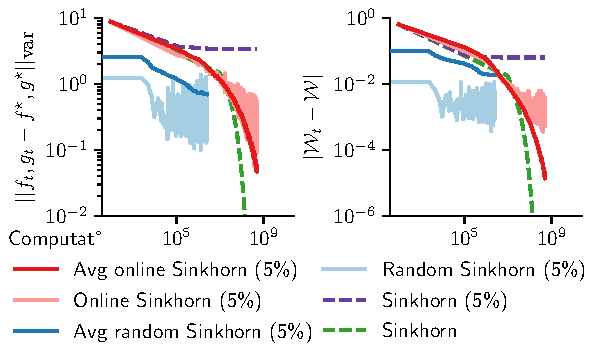
\includegraphics[width=\linewidth]{comparison.pdf}

    \vspace{-1em}

    \caption{Comparison of online, random and fixed sampling Sinkhorn performances. Online Sinkhorn overcomes the bias of sampling---especially with out-of-loop averaging. Random Sinkhorn gives fast estimations, whose variance does not decrease.}
    \label{fig:convergence}
\end{figure}


We first consider a discrete distribution $(\alpha, \beta)$, to be able to
compute the reference distance $\Ww = \Ww(\alpha, \beta)$ and the optimal potentials $f^\star$,
$g^\star$, using Sinkhorn algorithm. The goal here is not to perform better
than the Sinkhorn algorithm in the long run. Indeed, the constraints of online
Sinkhorn impose unnecessary slow-downs when dealing with small discrete
distributions. Rather, our purpose is to illustrate the consistency of online
Sinkhorn. We choose $\alpha$ and $\beta$ to be two discrete 1-D distributions,
$\Xx=\RR$, sampled from the continuous densities displayed in
\autoref{fig:potentials}. We set $\varepsilon = 10^{-2} \max_{x,y}
C(x,y)$, where we use the squared Euclidean loss (regularized $\Ww_2$
setting)---the distributions $\alpha$ and $\beta$ have bounded support. We use
$\eta_t = \frac{1}{\sqrt{t}}$ for online Sinkhorn and a fixed batch-size $n$, in
all experiments. We compare the performance of Sinkhorn, online Sinkhorn and
random Sinkhorn, measuring $\Vert f - f^\star \Vert_{\text{var}} + \Vert g -
g^\star \Vert_{\text{var}}$ and the absolute error $| \Ww_t - \Ww |$ versus the
number of computations performed--- the evaluation of $C(x_i, y_i)$ and the
computation of each addition in the $C$-transform being considered as elementary
computation units. We further report the performance of using out-of-loop
averaging with $\gamma_t = \frac{1}{\sqrt{t}}$.

\paragraph{Results.} We report convergence curves in \autoref{fig:convergence}.
Compared to the subsampled Sinkhorn algorithm that computes a biased estimate of
the distance $\Ww$ (purple), the online Sinkhorn algorithm successfully
estimates the distance and the associated potentials, despite performing only
partial $C$-transforms (red). Random Sinkhorn (blue) finds a decent estimation
of the distance and potentials, with fewer computations than the full Sinkhorn
algorithm, but fails to converge. Averaging the random Sinkhorn iterations finds
a biased estimation. The vanilla online Sinkhorn converges towards the true
value, albeit with a rather high iterate variance (note that this variance does
reduce---this is a log-log plot). Remarkably, the out-of-loop averaging of
online Sinkhorn enjoys much better converging property---we confirmed this
finding on many synthetic problems. It is surprising that an averaging mechanism
brings speed-up in a non-convex setting---we attribute this to the convexity of
the original problem, although this should be further investigated.

\begin{figure}[t]
    \centering
    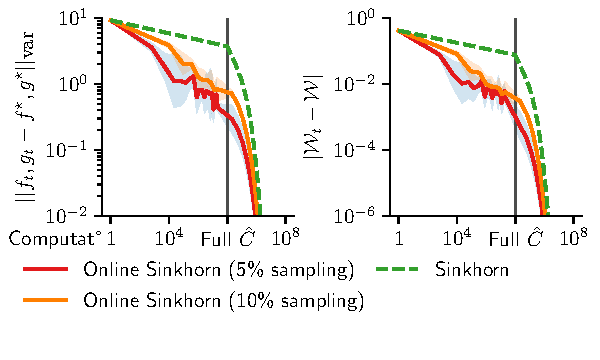
\includegraphics[width=\linewidth]{early_compute}
    
    \vspace{-1em}

    \caption{Using online Sinkhorn during the initial computation of the cost
     matrix accelerates the Sinkhorn algorithm: it provides good estimates of
     the potentials $f$ and $g$ to warm start the full Sinkhorn algorithm.
     Curves averaged over 5 runs. \label{fig:early_compute}}
\end{figure}

\begin{figure*}[t]
    \centering
    \if\icml0
    \begin{widepage}
    \fi
    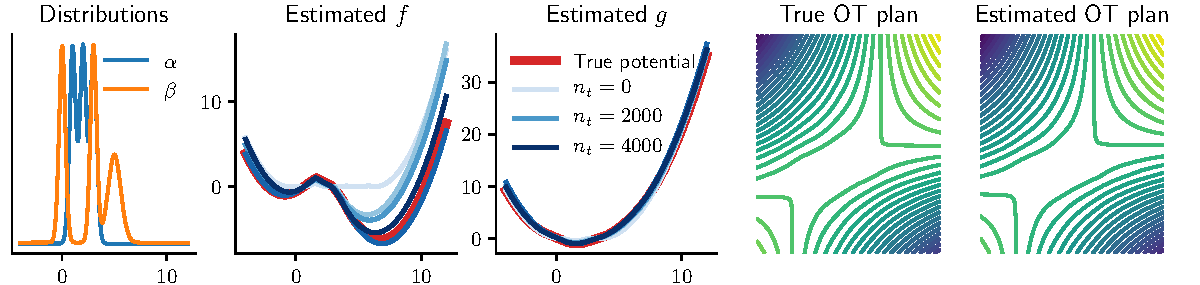
\includegraphics[width=\linewidth]{continuous.pdf}
    \caption{Representation of the convergence path of online Sinkhorn: the blue curves represents the estimated potentials (continuous functions) at different stages of the algorithm. The estimated plan $\pi_t$ is very quickly accurate, while the shape of the potentials match nearly perfectly the true potentials (estimated on a grid $N = 5000$). $\varepsilon = 10^{-2} \max \hat C$.
    \label{fig:potentials}
    }
    \if\icml0
    \end{widepage}
    \fi
\end{figure*}

\subsection{Accelerating the first Sinkhorn iteration}\label{sec:accelerating}

The discrete Sinkhorn algorithm requires to compute a full matrix $\hat C \eqdef
(C(x_i,y_i))_{i,j}$  of size $N \times N$, prior to estimating the
potentials $f_1$ and $g_1$ by a first $C$-transform. In contrast, online Sinkhorn can progressively
computes this matrix while computing first sketches of the potentials. We therefore
assess the performance of the following \textit{online+full Sinkhorn} algorithm
in a discrete setting: online Sinkhorn is run with batch-size $n$ during the first iterations, until
observing each sample of $[1,N]$, i.e. until the cost matrix $C$ is completely evaluated.
At this point (iteration $t$), online Sinkhorn provides the estimates $f_{t},
g_{t}$. From then, the algorithm only performs full Sinkhorn updates.


\paragraph{Results.} We report convergence curves in
\autoref{fig:early_compute}. The proposed scheme indeed provides an improvement
upon Sinkhorn algorithm. After $N^2$ computation (the cost of estimating the
full matrix $\hat C$), both the function value and distance to optimum are lower
using our scheme: the full Sinkhorn algorithm then operates from a good
initialization for potentials. Computing those cost approximately as much as
estimating the matrix $\hat C$ in dimension $1$. The \textit{online+full}
Sinkhorn algorithm then maintains an advantage over the full Sinkhorn algorithm
over time. Note that the cost of estimating initial potentials becomes negligible
as the dimension increase---the cost of computing $\hat C$ dominates. This
strongly advocates for using an online scheme as a warm-up for regularized OT
estimation. We note that using smaller batch-size $n$ may lead to higher speed-up (here, $n=50$ performs better than $n=100$).
There is an optimal $n$. The speed gain decreases with $\epsilon$, but remains
significant even for $\epsilon = 10^{-4} \max \hat C$. We add that
using a sampling-without-replacement scheme brings an additional speed-up. Out-of-loop averaging is also beneficial. We refer to the appendix for additional figures.

\subsection{Continuous potential estimation}

Finally, we measure the performance of our algorithm in a truly continuous
setting, where $\alpha$ and $\beta$ are $1$-D parametric distributions (Gaussian
mixtures) from which we sample. In the absence of reference $\Ww$ (which cannot be accurately computed
without a method akin to ours), we monitor the
trajectories of the potentials, and compare them to the Sinkhorn potentials for
realization of $\alpha$ and $\beta$ of size $n=2000$. We also monitor the
estimated transportation plan $\hat \pi_t = (\alpha \otimes \beta)
\exp(\frac{f\oplus g - C}{\varepsilon}) \in \Mm^+(\Xx)^2$. We run the experiments with
$n_T=5000$.

\paragraph{Results.} We show the convergence trajectories of the potentials in
\autoref{fig:potentials}. Online Sinkhorn refines the potentials $(f_t, g_t)_t$ until convergence. The fact that our method uses an adapted potential parametrization~\eqref{eq:param}
allows the iterates to quickly identify the correct shape of the optimum. The
final plan is undistinguishable from the true transportation plan. Quantitative
values (distance to true potentials, error in Sinkhorn distance estimation) converge as in
\autoref{fig:convergence}.

\paragraph{Comparison to concurrent approaches.}\label{sec:compare}Finally, we compare online
Sinkhorn to constructing representations of Sinkhorn potentials using universal
RKHS \citep{2016-genevay-nips}. This competing approach sets $f_t(\cdot) =
\sum_{i=1}^{n_t} \alpha_t \kappa(\cdot, x_i)$ (and similarly for $g_t$), where $\kappa$ is
a reproducing kernel (typically a Gaussian). This differs significantly from the
representations that we propose, for which $\exp(-f_t)$, and not $f_t$, is
expressed as a kernel mixture. 
%
With RKHS representations of potentials, the
dual problem \eqref{eq:sinkhorn} can be solved using stochastic gradient
descent, with theoretical convergence guarantees. As advocated by the authors,
we run a grid search over the bandwidth parameter~$\sigma$ of the Gaussian kernel to select the best
performing runs. We set $n_T = 50000$, and $\epsilon = 10^{-1} \max C$. We could not successfully use the RKHS method for lower $\epsilon$.

We compare the final potentials and associated transportation plans in
\autoref{fig:comparison_rkhs}. Our method estimates potentials with much less
errors, especially in areas where the mass of $\alpha$ and $\beta$ is low. The
computational complexity of both algorithms are comparable. Online Sinkhorn does
not require to set any hyperparameters, whereas we observed that SGD in RKHS is very
sensitive to bandwidth selection.

\begin{figure}[t]
    \centering
    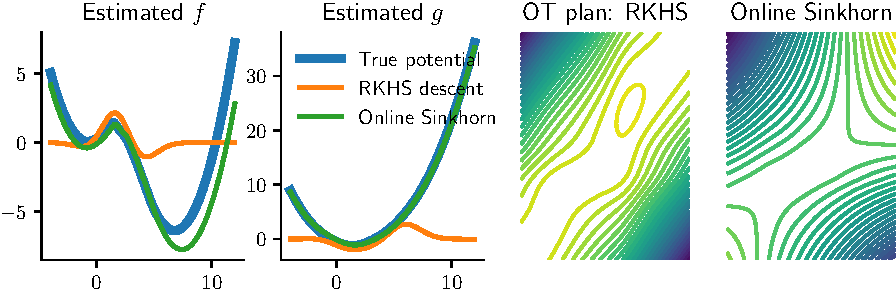
\includegraphics[width=\linewidth]{continuous_francis-crop.pdf}
    \caption{Comparing online Sinkhorn with SGD over a RKHS representation of the potential \citep{2016-genevay-nips}, with best bandwidth parameter. Online Sinkhorn finds more accurate functional representations of potentials, thanks to its more appropriate parametrization. $\varepsilon = 10^{-1} \max \hat C$.}
    \label{fig:comparison_rkhs}
\end{figure}

%!TEX root = article.tex

\section{Conclusion}

We have extended the classical Sinkhorn algorithm to cope with streaming samples. The resulting online algorithm computes a non-parametric expansion of the inverse scaling variables using kernel functions. In contrast with previous attempts to compute OT between continuous densities, these kernel expansions fit perfectly the structure of the entropic regularization, which is key to the practical efficiently of our method. 
%
We have drawn links between regularized OT and stochastic approximation. This opens promising avenues to study convergence rates of continuous variants of Sinkhorn's iterations, with a further refinements of the constants



% \section{Acknowledgements}
% This work was supported by the European Research Council (ERC project NORIA).

\pagebreak

\bibliography{biblio}
\bibliographystyle{icml2020}

\onecolumn

\appendix

\end{document}